%\documentclass[final]{article}
\documentclass[]{article}
\usepackage{geometry}
\geometry{
	a4paper,
	total={170mm,257mm},
	left=0.75in,
	top=0.75in,
	right=0.75in,
	bottom=1in,
}
\newcommand{\extramargin}[1]{}
%\newcommand{\extramargin}[1]{
	%	\setlength{\paperwidth}{250mm}
	%	\setlength{\evensidemargin}{-15mm}
	%	\setlength{\oddsidemargin}{-15mm}
	%}
\usepackage{gensymb}
\usepackage{lipsum}
\usepackage{graphicx}
\usepackage{epstopdf, epsfig}
\usepackage{amsmath}
\usepackage[url=false,
backend=bibtex,
style=authoryear-comp,
giveninits=true,
doi=true,
isbn=true,
backref=false,
dashed=false,
maxcitenames=2,
maxbibnames=99,
natbib=true]{biblatex}
\DeclareNameAlias{author}{last-first}
\DeclareFieldFormat
[article,inbook,incollection,inproceedings,patent,thesis,
unpublished,techreport,misc,book]
{title}{#1}
\renewcommand*{\revsdnamepunct}{}
\renewbibmacro{in:}{}
\usepackage{xpatch}
\xpatchbibmacro{date+extradate}{%
	\printtext[parens]%
}{%
	\setunit*{\space}%
	\printtext%
}{}{} 


\addbibresource{../Main/ViscousDropImpact_v2.bib}
\nonfrenchspacing
\setlength\parindent{0pt}
\usepackage{siunitx}
\usepackage{xcolor}
\usepackage{mathrsfs}
\usepackage[colorlinks,citecolor=purple]{hyperref}
\newcommand*\blue{\textcolor{blue}}
\newcommand*\red{\textcolor{red}}
\newcommand{\VS}[1]{{\textcolor{orange}{#1}}}

\renewcommand{\thefigure}{R\arabic{figure}}

\usepackage[obeyFinal,colorinlistoftodos, textwidth=60mm, shadow]{todonotes}
% todonotes specific macros begin!
\newcommand{\todoInsertref}[2]{\todo[color=green!40, #1]{#2}}
\newcommand{\todoExplaininDetails}[2]{\todo[color=orange!40, #1]{#2}}
\newcommand{\todoUrgent}[2]{\todo[color=red!40, #1]{#2}}
\newcommand{\todoSansUrgent}[2]{\todo[color=yellow!40, #1]{#2}}
\extramargin
%% todonotes specific macros end!

%opening
\title{Reply to Referee 2}
\author{Vatsal Sanjay, Bin Zhang, Cunjing Lv, and Detlef Lohse}
\date{}
\begin{document}
	
\maketitle
	
\textit{The manuscript ``Inertia \& viscosity dictate drop impact forces," by Sanjay and coauthors, reports experimental and numerical evidence of drop impact under a wide range of conditions, covering cases in which surface tension, viscosity, or inertia become dominant. Their main focus is understanding the laws that govern the primary and secondary peak of force signals, $F_1$ and $F_2$, and the times at which they occur, $t_1$ and $t_2$. The authors provide physical arguments that elucidate the data dependency on two dimensionless control parameters, the Weber ($We$) and the Ohnesorge ($Oh$) number, establishing general scaling laws. The physics of several limiting cases is also described in detail, fulfilling a broad picture of the studied quantities in the space of parameters.}
		
\textit{This work addresses a profound and relevant question regarding drop impact, which has implications for many applications. To improve our understanding of the involved physical quantities, the authors perform and report several new experiments and simulations, extending the range of parameters of gathered data. Accordingly, the manuscript presents a regime map for the force peaks, constituting its main contribution. Thus, The goal is well-aimed, and evidence and theory support the results well. However, I still have some concerns that I include in the attached report, which the authors should address to assert and clarify several claims in the manuscript.}
	
\textit{The manuscript is well-structured, easy to understand, and phrased in excellent English. Figures are not only helpful but also beautiful. The authors disclose every necessary detail to understand the experiments and numerical simulations and how they complement. Also, the literature on this problem cited in the manuscript is comprehensive.}
	
\textit{In summary, this manuscript that studies the drop-impact force peaks dependency on Weber and Ohnesorge numbers provides new and relevant data and contributes with a necessary regime map on each of the quantities examined and in a broader range of the dimensionless number under study. I will be eager to recommend its publication in the Journal of Fluid Mechanics after the authors solve the points I raised in the attached report.}\\[2mm]

We thank the referee for carefully reading our manuscript and providing valuable feedback and suggestions. We have reviewed the referee's comments and made changes based on their suggestions. Below, we offer a point-to-point reply to each of the referee's comments and include the changes made in the manuscript. The referee's comments are in italics, and our replies are in plain black. Changes in the manuscript are highlighted in orange.

\begin{enumerate}
	\item \textit{Line1: The title is misleading. As far as I understand,both $F_1$ and $F_2$, and $\tau_1$ and $\tau_2$, depend under some regimes on surface tension $\gamma$, but the title excludes surface tension as a relevant parameter in drop impact forces. Authors could explain this better or choose a title that reflects all the quantities under study.}
	
	We agree with the reviewer that the title was misleading. Of course, all three: inertia, capillarity, and viscosity, play a role. Indeed, we have studied the role of inertial and capillarity in \citet{zhang2022impact}. We have now changed the title of the paper to:
	
	\VS{The role of viscosity on drop impact forces}
	
	\item \textit{Figure 2: Although there are several pressure and velocity maps, etc., to characterize the different regimes throughout the article, there is only a single force signal (figure 2). Would the article benefit from including force signals for at least limiting cases of the dimensionless parameters? Force signal, the easier way to experimentally characterize the phenomenon, should provide a simple signature of the regime at which the drop impact occurs.}
	
	 We thank the reviewer for this remark. To extend the comparison at different Ohnesorge numbers $Oh$, we have added two additional $F(t)$ curves in figure 2 (see figure~\ref{fig:summary}). Furthermore, throughout the manuscript, we present experimental data wherever available (see figures 3 and 7). 
	 
	 	\begin{figure}
	 	\centering
	 	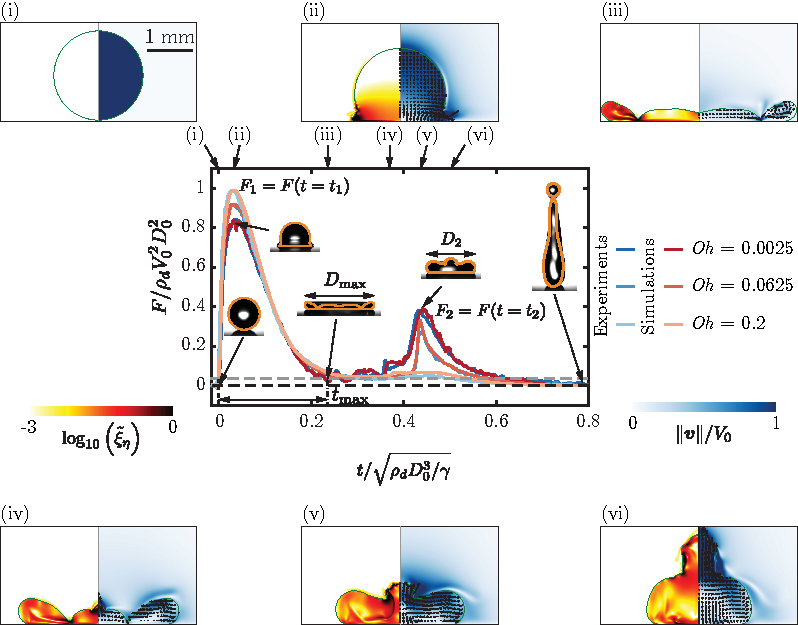
\includegraphics[width=\textwidth]{../Main/Figures/Figure1_summary_v5.pdf}
	 	\caption{\VS{Comparison of the drop impact force $F(t)$ obtained from experiments and simulations for the three typical cases with impact velocity $V_0 = 1.2\,\si{\meter}/\si{\second}, 0.97\,\si{\meter}/\si{\second}, 0.96\,\si{\meter}/\si{\second}$, diameter $D_0 = 2.05\,\si{\milli\meter}, 2.52\,\si{\milli\meter}, 2.54\,\si{\milli\meter}$, surface tension $\gamma = 72\,\si{\milli\newton}/\si{\meter}, 61\,\si{\milli\newton}/\si{\meter}, 61\,\si{\milli\newton}/\si{\meter}$ and viscosity $\eta_d = 1\,\si{\milli\pascal\second}, 25.3\,\si{\milli\pascal\second}, 80.2\,\si{\milli\pascal\second}$. These parameter give $Oh = 0.0025, 0.0625, 0.2$ and $We = 40$.
		For the three cases, the two peak amplitudes, $F_1/\rho_dV_0^2D_0^2 \approx$ 0.82, 0.92, 0.99 at $t_1 \approx 0.03\sqrt{\rho_dD_0^3/\gamma}$ and $F_2/\rho_dV_0^2D_0^2 \approx$ 0.37, 0.337, 0.1 at $t_2 \approx 0.42\sqrt{\rho_dD_0^3/\gamma}$, characterize the inertial shock from impact and the Worthington jet before takeoff, respectively. 
		The drop reaches the maximum spreading at $t_{\text{max}}$ when it momentarily stops and retracts until $t_3 \approx 0.8\sqrt{\rho_dD_0^3/\gamma}$ when the drop takes off ($F = 0$).
		Six instances are further elaborated through numerical simulations for ($We = 40, Oh = 0.0025$), namely (i) $t = 0\,\si{\milli\second}$ (touch-down), (ii) $t = 0.37\,\si{\milli\second}$ ($t_1$), (iii) $t = 2.5\,\si{\milli\second}$ ($t_{\text{max}}$), (iv) $t = 3.93\,\si{\milli\second}$ ($\approx 0.85t_2$), (v) $t = 4.63\,\si{\milli\second}$ ($t_2$), and (vi) $t = 5.25\,\si{\milli\second}$ ($\approx 1.15t_2$). 
		We stress the excellent agreement between experiments and simulations without any free parameters. The insets show representative snapshots at specific time instants overlaid with the drop boundaries from simulations in orange, also revealing good agreement. 
		The left part of each numerical snapshot shows the dimensionless local viscous dissipation function $\tilde{\xi}_\eta \equiv \xi_\eta D_0/\left(\rho_dV_0^3\right) = 2Oh\left(\boldsymbol{\tilde{\mathcal{D}}:\tilde{\mathcal{D}}}\right)$, where, $\boldsymbol{\mathcal{D}}$ is the symmetric part of the velocity gradient tensor, on a $\log_{10}$ scale and the right part the velocity field magnitude normalized with the impact velocity. The black velocity vectors are plotted in the center of mass reference frame of the drop to clearly elucidate the internal flow.}}
	 	\label{fig:summary}
	 \end{figure}
	 
	 \begin{figure}
	 	\centering
	 	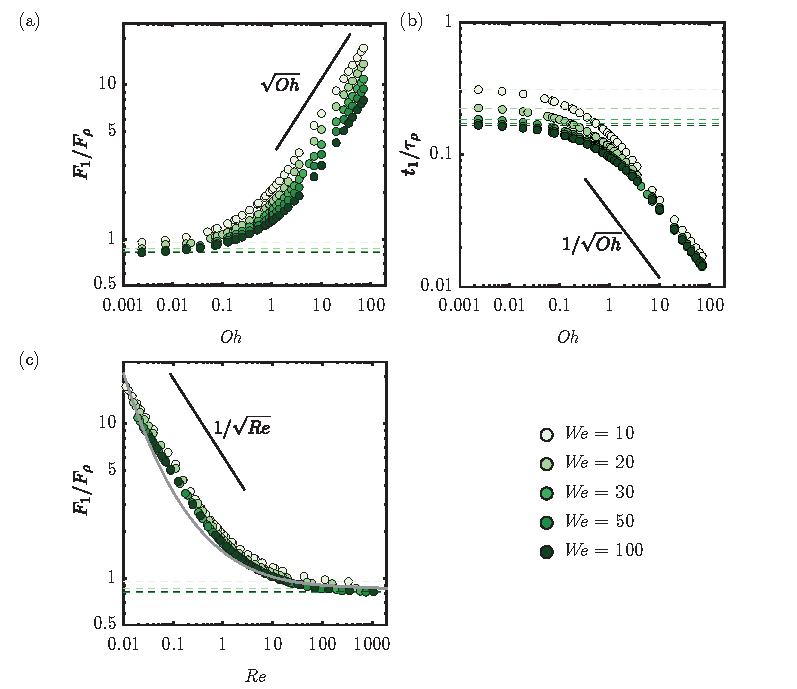
\includegraphics[width=\textwidth]{../main/Figures/ForceTimeVersusOhnesorge.pdf}
	 	\caption{\blue{Anatomy of the first impact force peak amplitude for viscous impacts from our numerical simulations: the $Oh$ dependence of  (a) the magnitude $F_1$ normalized by the inertial force scale $\rho_dV_0^2D_0^2$ and (b) the time $t_1$ to reach the first force peak amplitude normalized by inertial timescale $\tau_\rho = D_0/V_0$}. \VS{(c) The $Re$ dependence of the magnitude $F_1$ normalized by the inertial force scale $\rho_dV_0^2D_0^2$ as compared to the (implicit) theoretical calculation of \citet{Gordillo2018}.} \blue{The black line corresponds to the scaling relationship described in \S~3.2. The Weber number is color-coded.}}
	 	\label{fig:F1Anatomy_2}
	 \end{figure}
	 
	 \item 
	 \begin{enumerate}
	 	 \item \textit{Line111-114: Previous studies have considered much broader ranges of viscosities (c.f. Cheng 2022 and references therein) using other liquids and solutions. Readers could be addressed for completeness.}
	 	\item \textit{Figure 5: The authors of several other studies have found that $F1/F_\rho$ depends solely on the Reynolds number (Re), collapsing curves in an extensive range of high Re numbers. Have the authors tried to remove the dependency on $\gamma$ (through Oh)? Since $Re \equiv \frac{\sqrt{We}}{Oh}$, I wonder if using it could collapse curves, at least in the low Oh limit.}	 	
	 \end{enumerate}
	 	
	Using water-glycerol mixtures allows us to probe two orders of magnitude in $Oh$ in the experiments. In the hindsight of finishing this project, we agree with the reviewer that using other liquids (such as silicone oil) will allow one to probe a wider range of viscosity  (and hence $Oh$). Of course, such liquids cannot be used with the superhydrophobic surfaces that we use in our work but would require superamphiphobic surfaces, such as the ones used in \citet{deng2012candle, ramirez2020lifting}. We have added this remark in the revised manuscript. 
	
	\S~\red{2.1:}\\
	\VS{We note that using other liquids like silicone oil could allow for a wider range of viscosity variation if used with a superamphiphobic substrate \citep{deng2012candle}.}
	
	Unfortunately, we do not have experiments for $Oh \gg 1$ (figure 5). Nonetheless, we can compare our results with those in \citet{Gordillo2018, cheng2021drop} illustrating $F_1(Re)$, where $Re = V_0D_0/\nu_d$ is the impact Reynolds number. We were, indeed, able to collapse the data for low $Re$ (high $Oh$) limit. there is still some scatter at high $Re$ (low $Oh$) owing to the $We$ dependence of the impact force peak amplitude. We have added this as figure 5(c). 
	
	\S~\red{3.2:}\\
	\VS{Figure~5 further shows that these scaling laws are weakly dependent on the Weber number, as viscous dissipation consumes the entire initial kinetic energy of the impacting drop (figure~6). Once again, we stress that using the water-glycerol mixtures limits the range of $Oh$ that we can probe experimentally. 
	We further note that the first peak is robust and does not depend on the wettability of the substrate. Consequently, to compare with the existing data such as those in \citet{cheng2021drop} with different liquids to cover a wider range of liquid viscosities and to account for the apparent $We$-dependence, we plot $F_1$ compensated with $F_\rho$ against the impact Reynolds number $Re \equiv \frac{\sqrt{We}}{Oh} = V_0D_0/\nu_d$. 
	For the low $Re$ regime, such a plot allows us to describe the $We$ dependence on the prefactor more effectively, as illustrated in figure~5(c). However, it is important to note that some scatter is still observed at high $Re$ values, which can be attributed to the $We$ dependence of the impact force peak amplitude. This lack of a pure scaling behavior demonstrates how the interplay between kinetic energy and viscous dissipation within the drop dictates the functional dependence of the maximum impact force on $Oh$.}
	
	
	\item
	\begin{enumerate}
		\item \textit{Eq. 3.4: Following previous comments, results in the literature (e.g., Cheng 2022) include corrections as a function of Re in the low Re limit. Have the authors tried adding them to their expression to include both viscous and capillary contributions?}
		\item \textit{Eq.~3.7: I am still not convinced of the validity of averaging over $t_{\text{max}}$ in Eq.~3.7. Many assumptions under consideration are valid only for the early impact and not through the spreading regime, which scales as $t_{\text{max}}$. In order to convince the readers, authors need to address this.}
	\end{enumerate}
	
	Thank you for raising this important point about the use of the $t_{\text{max}}$ as the timescale for impact in the large Ohnesorge number ($Oh$) regime. We appreciate the opportunity to clarify our approach and present the modifications made to the theoretical model based on your critique and our recent work \citep{sanjay2024PRL}.
	
	In the revised version of the manuscript, we have made two major changes to the model:
	
	\begin{enumerate}
		\item[$\bullet$] We now integrate until $\tau_\rho$ instead of $t_{\text{max}}$, as you correctly pointed out. The first peak appears within a fraction of $t \sim \tau_\rho$ (see Figures 3 and 4).
		\item[$\bullet$] For the viscous regime, we propose that the entire initial kinetic energy is lost from $t = 0$ until $t = \tau_\rho = D_0/V_0$. The viscous dissipation during this time frame dictates the drop impact force.
	\end{enumerate}
	
	With these modifications, the leading order of the model now gives $F_1 \sim 1/\sqrt{Re}$ (see Figure 5c of the revised manuscript or Figure~\ref{fig:F1Anatomy_2} of this reply). This result is consistent with the findings of \citet{Gordillo2018}. In fact, there is only a minor discrepancy between the theoretical results of \citet{Gordillo2018, cheng2021drop} and our direct numerical simulation data.
	
	However, we still recommend the need for a predictive model to obtain the first force peak amplitude $F_1$ based on the control parameters $We$ and $Oh$. We address this question in our recent work \citep{sanjay2024PRL}, where we use global energy balances to unify the scaling of drop impact forces in different parts of the parameter space. We have also added a brief discussion of this in the revised manuscript.
	
	\S~\red{5:}\\
	\VS{Although, the implicit theoretical model summarized in \citet{cheng2021drop} describes most of data in figure~5, we stress the importance of having a predictive model to determine $F_1$ for given $We$ and $Oh$ \citep{sanjay2024PRL}.} 
	
	\S~\red{3.2:}\\
	\blue{To systematically elucidate these scaling behaviors in the limit of small $Re$, we need to find the typical scales for the rate of change of kinetic energy and that of the rate of viscous dissipation for the drop impact system. First, we can readily define an average rate of viscous dissipation per unit mass as}
	
	\blue{\begin{align}
			\bar{\varepsilon} \sim \frac{1}{\tau_\rho}\frac{1}{D_0^3}\int_0^{\tau_\rho}\int_\Omega\nu_d\left(\boldsymbol{\mathcal{D}:\mathcal{D}}\right)d\Omega dt,
	\end{align}}
	
	\noindent \blue{where $\nu_d$ is the kinematic viscosity of the drop and $d\Omega$ is the volume element where dissipation occurs. Notice that $\bar{\varepsilon}$ has the dimensions of $V_0^3/D_0$, i.e., length squared over time cubed or velocity squared over time, as it should be for dissipation rate of energy per unit mass. We can estimate $\Omega = D_{\text{foot}}^2l_\nu$ (figure~6), where $D_{\text{foot}}$ is the drop's foot diameter in contact with the substrate and $l_\nu$ is the viscous boundary layer thickness.} \VS{This boundary layer marks the region of strong velocity gradients ($\sim V_0/l_\nu$) analogous to the \citet{mirels1955laminar} shockwave-induced boundary layer. For details, we refer the authors to \citet{schlichting2016boundary, Schroll2010, Philippi2016}. Consequently, the viscous dissipation rate scales as}
	
	\blue{\begin{align}\label{eq:dissipationScale}
			\bar{\varepsilon} \sim \frac{1}{\tau_\rho D_0^3}\int_0^{\tau_\rho}\nu_d \left(\frac{V_0}{l_\nu}\right)^2 D_{\text{foot}}^2l_\nu dt.
	\end{align}}
	
	\noindent \blue{To calculate $D_{\text{foot}}$, we assume that the drop maintains a spherical cap shape throughout the impact (figure~6). To calculate the distance the drop would have traveled if there were no substrate, we use the relation $d \sim V_0t$. Simple geometric arguments allow us to determine the relation between the foot diameter and this distance, $D_{\text{foot}} \sim \sqrt{D_0d}$ \citep{lesser1981analytic, mandre2009precursors,  zheng2021air, bilotto2023fluid, bertin2023similarity}.} \VS{Interestingly, this scaling behavior is similar to the inertial limit \citep{wagner1932stoss, Bouwhuis2012, Philippi2016, gordillo2019theory} as discussed by \citet{langley2017impact, bilotto2023fluid}.} \blue{Furthermore, the viscous boundary layer $l_\nu$ can be approximated using $\sqrt{\nu_d t}$ \citep{mirels1955laminar, Eggers2010, Philippi2016}. Filling these in \eqref{eq:dissipationScale}, we get}
	
	\blue{\begin{align}	
			\bar{\varepsilon} \sim \frac{1}{\tau_\rho D_0^2}\int_0^{\tau_\rho}\sqrt{\nu_d} V_0^3 \sqrt{t} dt,
	\end{align}}
	
	\noindent \blue{which on integration gives}
	
	\VS{\begin{align}\label{eq:eps0Final}
			\bar{\varepsilon} \sim \sqrt{\nu_d \tau_\rho}V_0^3/D_0^2, 
	\end{align}}
	
	\noindent \VS{where $\tau_\rho$ is the inertial time scale. Here, we assume that for highly viscous drops, all energy is dissipated within a fraction of $\tau_\rho$. Filling in \eqref{eq:eps0Final} and normalizing $\bar{\varepsilon}$ with the inertial scales $V_0^3/D_0$,}
	
	\VS{\begin{align}\label{eq:DissipationScale}
			\frac{\bar{\varepsilon}}{V_0^3/D_0} \sim \sqrt{\frac{\nu_d\tau_\rho}{D_0^2}} = \frac{1}{\sqrt{Re}} = \left(\frac{Oh}{\sqrt{We}}\right)^{1/2}.
	\end{align}}
	
	\noindent \blue{Next, the kinetic energy of the falling drop is given by}
	
	\blue{\begin{align}\label{eq:KEdissipation}
			\dot{K}(t) \equiv \frac{dK(t)}{dt} \sim \rho_dD_0^3\bar{\varepsilon},\quad\text{where } K(t) = \frac{1}{2}m\left(V(t)\right)^2,
	\end{align}}
	
	\noindent \blue{and $V(t)$ is the drop's center of mass velocity. The left-hand side of \eqref{eq:KEdissipation} can be written as}
	
	\blue{\begin{align}\label{eq:KE-powerTime}
			\dot{K}(t) = mV(t)\frac{dV(t)}{dt} = F(t)V(t).
	\end{align}}
	
	\noindent \blue{In equation~\eqref{eq:KE-powerTime}, $F(t)$ and $V(t)$ scale with the first impact force peak amplitude $F_1$ and the impact velocity $V_0$, respectively, giving the typical scale of the rate of change of kinetic energy as}
	
	\blue{\begin{align}\label{eq:KE-power}
			\dot{K}^* \sim F_1V_0.
	\end{align}}
	
	\noindent \blue{We stress that \eqref{eq:KE-power} states that the rate of change of kinetic energy is equal to the power of the normal reaction force, an observation already made by \citet{wagner1932stoss} and \citet{Philippi2016} in the context of impact problems. Lastly, at large $Oh$, viscous dissipation enervates kinetic energy completely giving (figure~6c, also see:  \citet{Philippi2016} and \citet{ Wildeman2016}),}
	
	\blue{\begin{align}\label{eq:force-Dissipation}
			\dot{K}^* \sim F_1V_0 \sim \rho_dD_0^3\bar{\varepsilon}
	\end{align}}
	
	\noindent \blue{Additionally, we use the inertial scales to non-dimensionalize  \eqref{eq:force-Dissipation} and fill in \eqref{eq:DissipationScale}, giving}
	
	\VS{\begin{align}
			\frac{F}{F_\rho} \sim \frac{\bar{\varepsilon}}{V_0^3/D_0} \sim \frac{1}{\sqrt{Re}} = \left(\frac{Oh}{\sqrt{We}}\right)^{1/2}
	\end{align}}
	
	\noindent \blue{and using $F_1t_1 \sim \rho_dV_0D_0^3 = F_\rho\tau_\rho$,}
	
	\VS{\begin{align}
			\frac{t_1}{\tau_\rho} \sim \left(\frac{\sqrt{We}}{Oh}\right)^{1/2}.
	\end{align}}
	
	\VS{In summary, we use energy and momentum invariance to elucidate the parameter dependencies of the impact force as illustrated in figure~5. The scaling arguments capture the dominant force balance during the impact process, considering the relative importance of inertial, capillary, and viscous forces. As the dimensionless viscosity of impacting drops increases, the lack of surface deformation increases the normal reaction force (3.16). Further, the invariance of incoming drop momentum implies that this increase in normal reaction force occurs on a shorter timescale (3.17).}
	
	\begin{figure}
		\centering
		\includegraphics[width=0.9\textwidth]{../main/Figures/RegimeMaps_v3.pdf}
		\caption{\blue{Regime map in terms of the drop Ohnesorge number $Oh$ and the impact Weber number $We$ to summarize the two peaks in the impact force by showing the different regimes described in this work based on (a) the first peak in the impact force peak amplitude $F_1$ and (b) the second peak in the impact force peak amplitude $F_2$. Both peaks are normalized by the inertial force scale $F_\rho = \rho_dV_0^2D_0^2$. These regime maps are constructed using $\sim 1500$ simulations in the range $0.001 \leq Oh \leq 100$ and $1 \leq We \leq 1000$.} \VS{The gray solid line in (a) and dashed line in (b) mark the inertial--viscous transition ($Re = 1$) and the bouncing--no-bouncing transition \citep[$Oh_c = 0.53$ for $Bo = 1$, see][]{sanjay_chantelot_lohse_2023}, respectively.}}
		\label{fig:RegimeMaps}
	\end{figure}

	\item \textit{As a suggestion, I find that adding a Reynolds-number (tilted) axis, which nicely follows the slope of the central transition area of the white region of inset (a), will help readers to place previous experimental results in this regime map. It may be redundant, but still very helpful.}\\[0.1mm]
	
	We thank the review for this suggestion. We have modified figure 10 to include $Re = 1$ transition line (see figure~\ref{fig:RegimeMaps}). 
	
\end{enumerate}	
	
\printbibliography[title=References]
\end{document}